
\documentclass[a4paper,12pt]{article}

\usepackage[a4paper, total={6in, 8in}, left=30mm]{geometry}
\usepackage{pdfpages}

\usepackage{cmap}
\usepackage[T2A]{fontenc}
\usepackage[utf8]{inputenc}
\usepackage[english,russian]{babel}
\usepackage{fancyhdr}
\usepackage{minted}
\usepackage{hyperref}
\usepackage{amsmath}
\usepackage[document]{ragged2e}

\hypersetup{
  colorlinks=true,
  linkcolor=black,
  urlcolor=blue,
  pdfborderstyle={/S/U/W 1}
}

\pagestyle{fancy}
\fancyhf{}
\lhead{Антон Завьялов, ПИ-72}
\rhead{\textbf{Расчетное задание}}
\cfoot{\thepage}

\makeatletter
\def\@seccntformat#1{%
  \expandafter\ifx\csname c@#1\endcsname\c@section\else
  \csname the#1\endcsname\quad
  \fi}
\makeatother

\begin{document} % Конец преамбулы, начало текста.
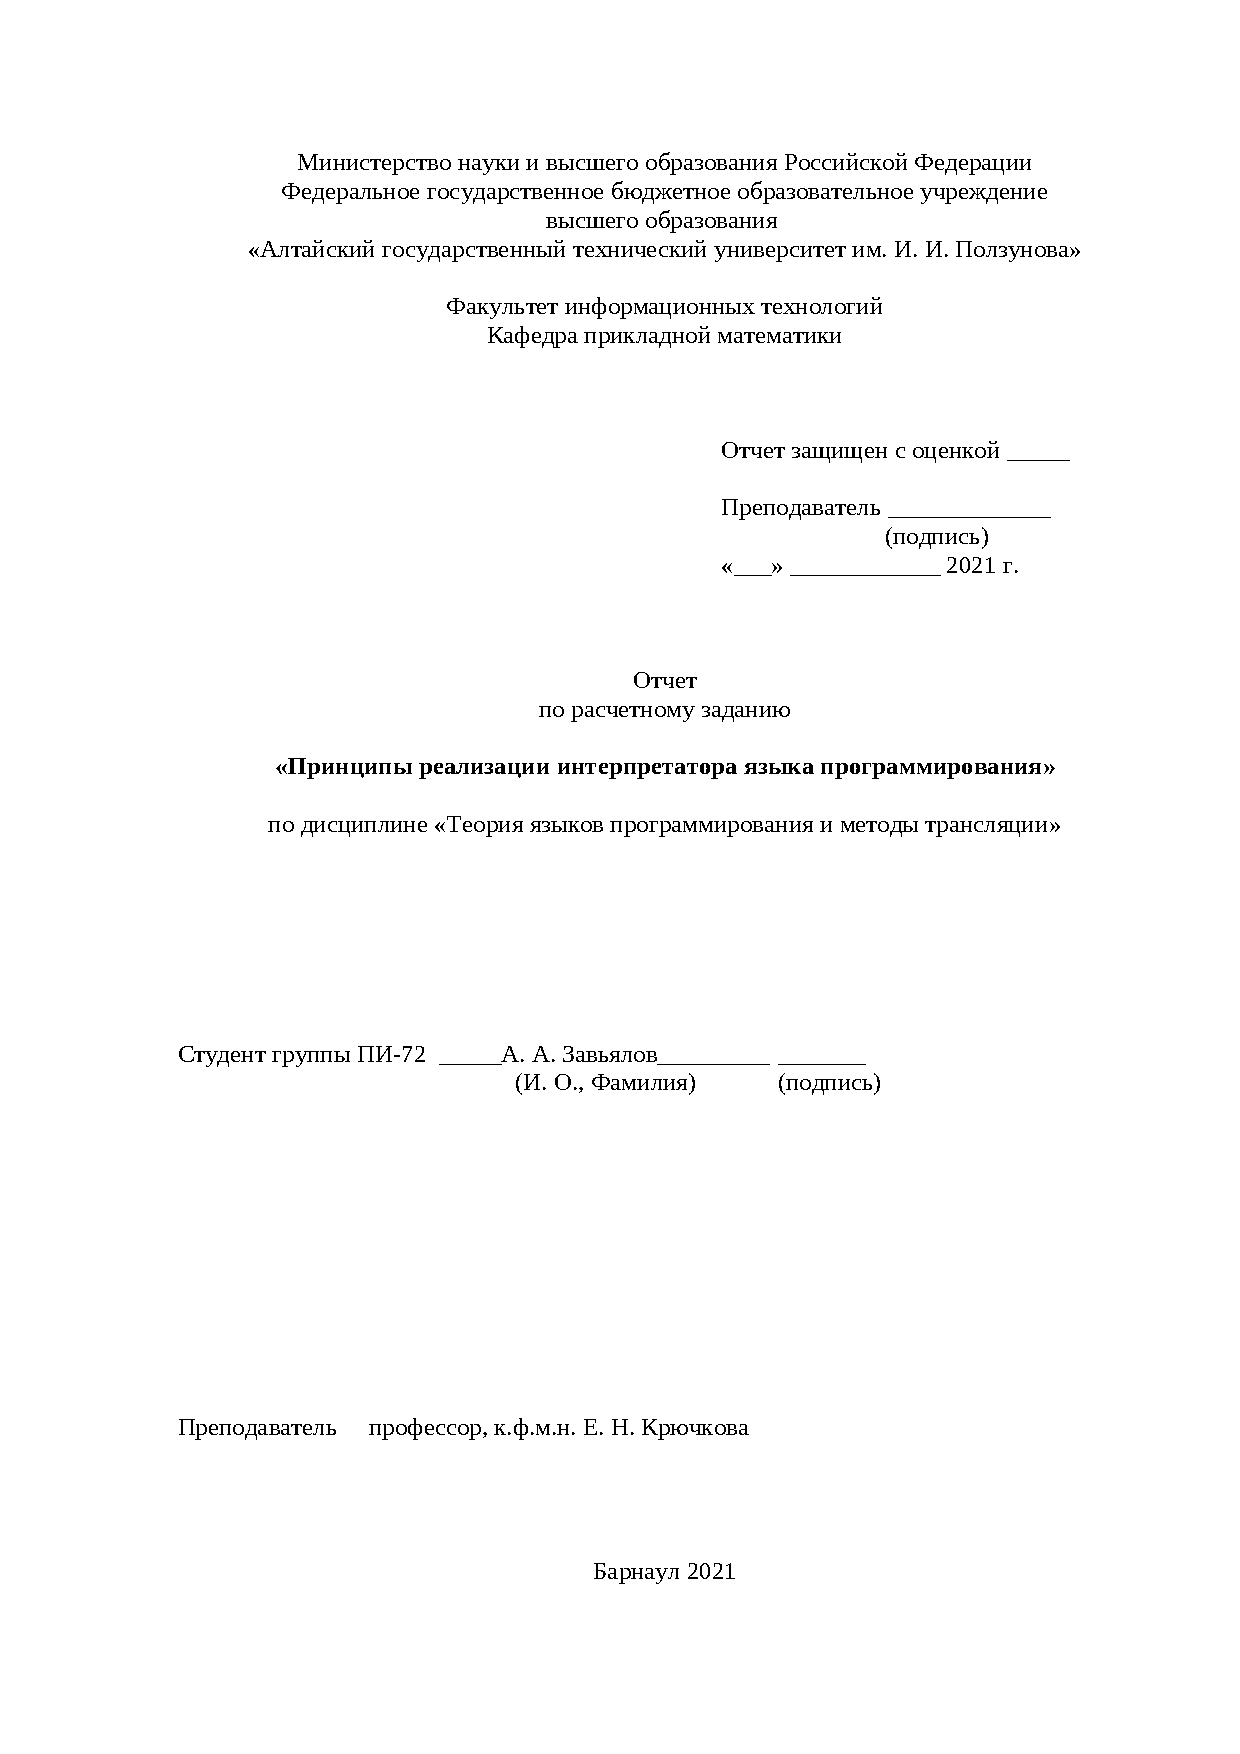
\includepdf[pages={1}]{title.pdf}

\tableofcontents
\newpage

\section{Тема расчетного задания}
\textbf{Принципы реализации интерпретатора языка программирования}
\begin{flushleft}
    \begin{itemize}
        \item Программа: класс Main  языка Java. Допускается описание внутренних классов. Методы классов не имеют параметров, но возвращают значение;
        \item Типы данных: int  (short  и  long), double;
        \item Операции: все арифметические, сравнения и логические;
        \item Операторы: присваивания и switch;
        \item Операнды: простые переменные, данные  классов  и константы;
        \item Константы:  целые  и вещественные  в экспоненциальной форме.
    \end{itemize}
\end{flushleft}
\newpage
\section{Типы данных языка и поле хранимых значений данных}
\begin{table}[h]
  \centering
  \begin{tabular}{|l|l|l|l|}
  \hline
      Тип & Объем кодирования & Имеет знак & Минимальное значение \\ \hline
      int & 32 бита (4 байта) & Да & -2\^31 \\ \hline
      short & 16 бит (2 байта) & Да & -32\_768 \\ \hline
      long & 64 бита (8 байт) & Да & -2\^63 \\ \hline
      double & 64 бита (8 байт) & Да & Согласно IEEE 754 \\ \hline
  \end{tabular}
  \begin{tabular}{|l|}
    \hline
        Максимальное значение \\ \hline
        2\^31 - 1 \\ \hline
        32\_767 \\ \hline
        2\^63 - 1 \\ \hline
        Согласно IEEE 754 \\ \hline
  \end{tabular}
\end{table}

\section{Способ хранения значений в семантической таблице для специальных конструкций}
\begin{flushleft}
  \begin{minted}[breaklines,frame=lines]{scala}
    // Простая переменная
    // tpe: тип значения (тэг размеченного объединения)
    // value: хранимое значение
    case class Variable(name: String, tpe: Type.Value, value: Any) extends SymbolNode
    
    // Поле класса
    // tpe: тип значения (тэг размеченного объединения)
    // value: хранимое значение
    case class Field(name: String, tpe: Type.Value, value: Any) extends SymbolNode
    
    // Метод
    // tpe: тип значения (тэг размеченного объединения)
    // value: возвращаемое значение
    case class Method(name: String, tpe: Type.Value, value: Any) extends SymbolNode
  \end{minted}
\end{flushleft}
\newpage
\section{СД, в которых выполняется выделение или освобождение памяти}
\begin{flushleft}
  \justify
  \begin{enumerate}
    \item Составной оператор (блок)
    Выделение памяти: выделяет память под все локальные ресурсы блока (переменные) на входе в блок; аллокация на стеке (способ выделения памяти полезно знать для генерации промежуточного кода в последующих работах).
    Освобождение памяти: освобождает память из-под всех локальных ресурсов при завершении блока; очищается кадр стека.
    \item Поле класса
    Выделение памяти: выделяет память под ресурс в абсолютно-адресованном пространстве при запуске программы (соответственно, при первом и единственном проходе синтаксического анализатора);
    Освобождение памяти: освобождается вместе с окружением программы во время завершения работы. Так как окружение и код программы выгружаются автоматически, нет необходимости освобождать память из-под полей вручную.
  \end{enumerate}
\end{flushleft}
\newpage
\section{СД, в которых выполняется вычисление значений}
\begin{flushleft}
  \justify
  \begin{enumerate}
    \item Унарная операция. 
    Унарный плюс и минус возвращают значение с соответствующим знаком.
    Отрицание, если операнд - 0 - возвращает 1, иначе возвращает 0.
    Инкремент, декремент, префиксные - увеличивают / уменьшают значение по ссылке на один и возвращают новое значение.
    Инкремент, декремент, постфиксные - сохраняют старое значение, увеличивают/уменьшают значение по ссылке и возвращают старое значение.
    \item Умножение/деление.
    Вычисляет произведение/частное двух операндов. Результат и семантика операции зависит от типов операндов - если один из операндов - число с плавающей точкой,
    используется арифметика с плавающей точкой, тип результата расширяется в соответствии с системой типов, спроектированной в прошлом семестре. В противном случае
    используется целочисленная арифметика.
    \item  Сложение/вычитание.
    Вычисляет сумму/разность двух операндов. На результат и семантику налагаются те же правила, как и в предыдущем пункте.
    \item Операции сравнения.
    Возвращает одно из двух чисел - 1 или 0 типа short, в зависимости от результата операции. На операции также налагается семантика расширения типа => 0 == 0.0 вернет true (1).
    (Опуская особенности IEEE 754)
    \item И и ИЛИ: 0 соответствует false, любые другие числа соответствуют true, вычисление аналогично C и Java, возвращается 1 или 0 типа short.
  \end{enumerate}
\end{flushleft}
\newpage
\section{СД, в которых используется флаг интерпретации}
\begin{flushleft}
  \justify
  \begin{enumerate}
    \item Метод.
    Если разбирается объявление метода, и метод не является точкой входа, при входе в блок метода отключается интерпретация, при выходе включается обратно.
    \item Оператор switch.
    Если оператор встретился во время интерпретации программы, на входе в switch интерпретация отключается, на выходе включается обратно (если до этого была включена).
    Если значение ветви совпадает с условием switch (в т.ч. если ветвь - стандартная (default)), и не был вызван break, интерпретация включается обратно.
    Если в ветви вызван break, интерпретация отключается до выхода из switch (текущего).
    \item Вызов метода и оператор return.
    Если во время интерпретации был вызван метод, сохраняется контекст исполнения (позиция сканера, текущий узел таблицы символов), текущим узлом семантического дерева
    становится узел, соответствующий определению метода, позиция сканера перемещается на начало блока метода. Поддерево блока привязывается к узлу определения метода
    особым образом - корню поддерева как родитель ставится определение метода, но определению метода не добавляются новые сыновья. Таким образом, разрешается область видимости,
    и не нарушается структура семантического дерева. Очевидно, что вызов возможен только в режиме интерпретации, так что изменять его не надо.

    Если во время разбора блока метода встретится return, интерпретация блока отключается до выхода из блока метода.

    При выходе из блока метода он уничтожается, ссылка на родителя заменяется на null, что избавляет от утечек памяти. При выходе из блока восстанавливаются позиция сканера,
    текущий узел семантического дерва.
    \item Простые операторы и операции.
    Если отключен режим интерпретации, переменным не присваиваются значения, не производятся арифметические вычисления, не происходит вывод информации в stdout при вызове println.
  \end{enumerate}
\end{flushleft}
\section{Проектирование способа отключения работы семантических подпрограмм при flagInterpret == false}
\begin{flushleft}
  \justify

Семантический анализ (проверка соответствия типов, разрешения имён и т.д.) нужен и без интерпретации программы, поэтому необходимо отключать только части, ответственные непосредственно за интерпретацию программы.

Проще и удобнее всего это сделать, изолируя главные и побочные эффекты интерпретации в конструкцию вида \textit{if (isInterpreting) \{ ... \}}


Например, в операторе присваивания при отключенном флаге интерпретации не будет присваивания значения и печати информации о присваивании:
\begin{minted}[breaklines,frame=lines]{scala}
  if (isInterpreting) {
    val lRef = l.asInstanceOf[Expr.Reference]
    // Присваивание значения по ссылке
    lRef.ref.value = SymbolNode.Type.cast(r.value, lRef.tpe)
    // Печать информации о присваивании
    println(s"${lRef.name} : ${lRef.tpe} = ${lRef.ref.value} : ${lRef.tpe}")
  }
\end{minted}
\end{flushleft}
\newpage
\section{Тесты и реакция программы интерпретатора}
\textbf{Тест на вычисление выражений}
\inputminted[breaklines,frame=lines,linenos]{java}{../src/test/fun-test/expressions/Correct.java}
Реакция программы:
\inputminted[breaklines,frame=lines,linenos]{text}{../src/test/fun-test/expressions/Correct.java.out}
\textbf{Тест на выполнение операций приведения типов}
\inputminted[breaklines,frame=lines,linenos]{java}{../src/test/fun-test/other/TypeCast.java}
Реакция программы:
\inputminted[breaklines,frame=lines,linenos]{text}{../src/test/fun-test/other/TypeCast.java.out}
\textbf{Тесты на работу операторов switch и break}

Тест на работу switch с break:
\inputminted[breaklines,frame=lines,linenos]{java}{../src/test/fun-test/statements/Switch.java}
Реакция программы:
\inputminted[breaklines,frame=lines,linenos]{text}{../src/test/fun-test/statements/Switch.java.out}
Тест на "проваливание" в ветви switch при отсутствии break:
\inputminted[breaklines,frame=lines,linenos]{java}{../src/test/fun-test/statements/Fallthrough.java}
Реакция программы:
\inputminted[breaklines,frame=lines,linenos]{text}{../src/test/fun-test/statements/Fallthrough.java.out}
Тест на частичное "проваливание" в ветви switch:
\inputminted[breaklines,frame=lines,linenos]{java}{../src/test/fun-test/statements/SemiFallthrough.java}
Реакция программы:
\inputminted[breaklines,frame=lines,linenos]{text}{../src/test/fun-test/statements/SemiFallthrough.java.out}
Тест на правильную работу return во вложенных операторах switch:
\inputminted[breaklines,frame=lines,linenos]{java}{../src/test/fun-test/statements/NestedSwitch.java}
Реакция программы:
\inputminted[breaklines,frame=lines,linenos]{text}{../src/test/fun-test/statements/NestedSwitch.java.out}
Тест на отключение интерпретации после вызова break в switch:
\inputminted[breaklines,frame=lines,linenos]{java}{../src/test/fun-test/statements/NoStatementsAfterBreak.java}
Реакция программы:
\inputminted[breaklines,frame=lines,linenos]{text}{../src/test/fun-test/statements/NoStatementsAfterBreak.java.out}
\textbf{Тесты на вызов методов и работу оператора return}

Тест на отключение интерпретации при определении методов:
\inputminted[breaklines,frame=lines,linenos]{java}{../src/test/fun-test/statements/MethodDefinition.java}
Реакция программы:
\inputminted[breaklines,frame=lines,linenos]{text}{../src/test/fun-test/statements/MethodDefinition.java.out}
Тест на вызов методов и сохранение контекста вложенных вызовов:
\inputminted[breaklines,frame=lines,linenos]{java}{../src/test/fun-test/statements/MethodCall.java}
Реакция программы:
\inputminted[breaklines,frame=lines,linenos]{text}{../src/test/fun-test/statements/MethodCall.java.out}
Тест на отключение интерпретации после вызова return:
\inputminted[breaklines,frame=lines,linenos]{java}{../src/test/fun-test/statements/NoStatementsAfterReturn.java}
Реакция программы:
\inputminted[breaklines,frame=lines,linenos]{text}{../src/test/fun-test/statements/NoStatementsAfterReturn.java.out}
Тест на правильную работу рекурсивных вызовов:
\inputminted[breaklines,frame=lines,linenos]{java}{../src/test/fun-test/statements/Recursion.java}
Реакция программы:
\inputminted[breaklines,frame=lines,linenos]{text}{../src/test/fun-test/statements/Recursion.java.out}
Тест на правильный возврат значений из методов:
\inputminted[breaklines,frame=lines,linenos]{java}{../src/test/fun-test/statements/ReturnValue.java}
Реакция программы:
\inputminted[breaklines,frame=lines,linenos]{text}{../src/test/fun-test/statements/ReturnValue.java.out}
\textbf{Тест на работу оператора присваивания}
\inputminted[breaklines,frame=lines,linenos]{java}{../src/test/fun-test/other/Assignment.java}
Реакция программы:
\inputminted[breaklines,frame=lines,linenos]{text}{../src/test/fun-test/other/Assignment.java.out}
\textbf{Тест интерпретации сложной программы}
\inputminted[breaklines,frame=lines,linenos]{java}{../src/test/fun-test/other/Complex.java}
Реакция программы:
\inputminted[breaklines,frame=lines,linenos]{text}{../src/test/fun-test/other/Complex.java.out}
\newpage
\section{Исходный код}
\begin{flushleft}
  Репозиторий с исходным кодом на GitHub: \url{https://github.com/andiogenes/very-smol-java-interpreter}
\end{flushleft}
\end{document}
